\begin{quote}
Вот уже некоторое время меня занимала идея написания книги о теории категорий,
предназначавшейся бы для программистов. Что характерно, не для учёных-информатиков,
а именно для программистов --- скорее инженеров, чем учёных. Понимаю, звучит это
довольно безумно, и я сам в должной мере напуган смелостью своей затеи. Нельзя отрицать,
что между наукой и инженерией лежит целая пропасть — уж я-то знаю, довелось поработать
с обеих её сторон. Но мне всегда жутко нравилось объяснять как работают разные штуки.
Необъятно моё восхищение Ричардом Фейнманом — подлинным мастером простых объяснений.
Я, конечно, не Фейнман, но я постараюсь изо всех сил.
Я начинаю с публикации этого вступления,
--- которое должно мотивировать читателя на изучение теории категорий
--- в надежде на начало дискуссии и получение обратной связи.\footnote{
    А ещё вы можете увидеть меня на видео, \href{https://www.youtube.com/playlist?list=PLbgaMIhjbmEnaH_LTkxLI7FMa2HsnawM_}{преподающим
    материал этой книги} живой аудитории.}
\end{quote}

\lettrine[lhang=0.17]{Я}{попытаюсь} в нескольких абзацах
убедить вас, что эта книга написана для вас, а все возражения, которые
у вас могут быть против изучения одной из самых абстрактных областей математики
в ваше ``обильное свободное время`` — абсолютно беспочвенны.

Мой оптимизм основывается на нескольких наблюдениях. Во-первых, теория категорий —
это настоящий клад крайне полезных для программирования идей. Программисты, использующие
Haskell, используют этот ресурс уже довольно давно, и идеи понемногу просачиваются
и в другие языки — но очень уж медленно. Надо бы нам его ускорить.

Во-вторых, математика бывает очень разная, и для очень разных аудиторий.
У вас может быть аллергия на матан или алгебру, но это ни в коем случае не
будет обозначать, что вы не получите удовольствия от теории категорий.
Я, пожалуй, даже возьму на себя смелость зайти довольно далеко, и сказать,
что теория категорий — это математика как раз того рода, что особенно идут
программистским умам. Причина в том, что теория категорий имеет дело не с
частностями, а с общей структурой. С той самой структурой, которая
позволяет нам компоновать программы.

Композиция находится в самом сердце теории категорий --- она является частью
определения понятия категории. Я же готов спорить, утверждая, что композиция
является самой сутью программирования. Композицией мы занимались всегда, задолго
до того как какому-то гениальному инженеру пришла в голову идея процедуры.
Когда-то принципы структурного программирования совершили в программировании
настоящую революцию, дав возможность компоновать программы из блоков кода.
Затем пришло объектно-ориентированное программирование, целиком и полностью
состоящее из композиции объектов. Функциональное программирование не только
компонует функции и алгебраические типы данных --- но и позволяет достичь
композиции многопоточности --- кое-чего практически невозможного при использовании
других парадигм программирования.

В-третьих, у меня есть секретное оружие: огромный мясницкий нож, при помощи которого
я уговорю математику стать более сговорчивой с программистами. Профессиональному
математику приходится быть очень осторожным, явно указывая все допущения,
маниакально соблюдая чёткость определений и старательно производя все доказательства.
Всё это делает математические книги практически недоступными для чтения человеком со стороны.
Сам же я по образованию физик, и в физике мы неоднократно добивались удивительного успеха,
используя довольно неформальные размышления. Математики смеялись над дельта-функцией Дирака,
сымпровизированной великим физиком Полем Дираком для решения дифференциальных уравнений
определённого рода. Но смех прекратился, когда формализация интуиции Дирака привела как
открытию абсолютно новой области математического анализа, называемой теорией обобщённых функций.

Разумеется, объясняя вещи на пальцах, всегда имеешь риск произнести какую-нибудь вопиющую чушь.
Поэтому я постараюсь удостовериться, что за каждым неформальным аргументом в этой книге стоит
твёрдая математическая теория. В конце концов, на моём ночном столике лежит изрядно повидавший виды
том "Теории категорий для работающего математика" самого Саундерса Маклейна.

Поскольку речь идёт о теории категорий \emph{для программистов}, я проиллюстрирую
все основные концепции программным кодом. Вы наверняка слышали, что функциональные языки
находятся куда ближе к математике, чем их более популярные императивные собратья.
Кроме того, они значительно мощнее в плане возможностей абстрагирования. Природным соблазном
было бы сказать: "До того как приступать к теории категорий вы должны выучить Haskell, иначе не получится!".
Но это бы значило, что за пределами мира функционального программирования теория категорий не имеет применения,
а это — попросту неправда. Так что будет куча примеров на C++. Само собой, придётся продираться через
уродливый синтаксис, логические шаблоны будет не так-то просто разглядеть на фоне многословности записи,
а вместо высокоуровневых абстракций может быть придётся что-нибудь и покопипастить — но что делать, такова уж
нелёгкая доля программирующего на C++.

Но и Haskell я упомянул не просто так. Профессиональными программистами на этом языке я вас становиться не заставлю,
но для набрасывания и документирования идей для дальнейшей имплементации на C++ он очень пригодится. Я, по крайней мере,
начал своё знакомство с Haskell именно таким образом. Его немногословный синтаксис и мощная система типов стали незаменимым
подспорьем для понимания и имплементирования шаблонов, структур данных и алгоритмов на C++. Однако, поскольку ожидать знания
Haskell от читателей я не могу, с ним мы будем знакомиться не торопясь, и я буду объяснять всё по ходу развития дела.

Если вы — опытный программист, вы можете уже спрашивать сами себя: сколько ж лет я уже программировал,
совершенно не волнуясь ни о какой теории категорий или функциональном подходе — и что, что изменилось вдруг?
Разумеется, трудно не заметить мощного потока фич из функциональных языков, захватывающего языки императивные.
Даже Java, этот бастион объектно-ориентированного подхода, пустила внутрь лямбда-функции. C++ последнее время
эволюционирует совершенно неистово --- новый стандарт выходит раз в пару лет --- пытаясь догнать стремительно
меняющийся мир. Вся эта активность происходит как подготовка к разрушительному изменению --- или, как называем его мы,
физики, фазовому переходу. Если достаточно долго нагревать воду, рано или поздно она закипит. Мы сейчас оказались в
положении той самой лягушки, которой предстоит решить: продолжать плавать во всё более тёплой воде, или начать искать альтернативы.

\begin{figure}
\centering
\fbox{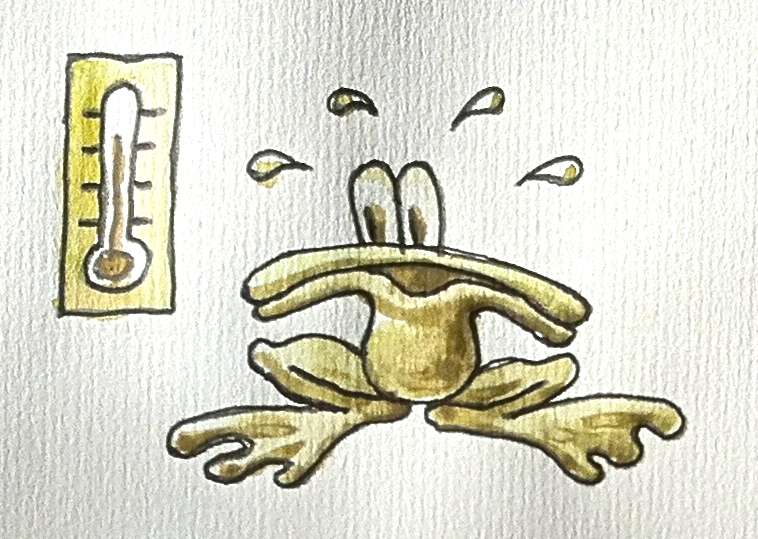
\includegraphics[width=3.12500in]{images/img_1299.jpg}}
\end{figure}

Одной из движущих сил этого великого изменения является революция многоядерных процессоров.
Превалирующая на данный момент парадигма объектно-ориентированного программирования, оказывается
практически бесполезной во вселенной многопоточности и параллелизма —-- хуже того, она поощряет опасные
архитектурные решения, чреватые трудноуловимыми багами. Сокрытие данных, основной компонент ОО-подхода,
в сочетании с совместным доступом к данным и их мутабельностью, образуют идеальный рецепт для ситуаций гонки.
Идея комбинирования мьютексов с защищаемыми ими данными, конечно, неплоха — да на беду композиции не поддаётся.
Кроме того, сокрытие примитивов синхронизации делает более вероятным и трудно отлаживаемым
возникновение ситуаций взаимной блокировки.

Но даже при рассмотрении вне контекста многопоточности, растущая сложность программных систем уже
проверяет на прочность пределы масштабируемости парадигмы императивного программирования. Проще говоря,
побочные эффекты уже совсем от рук отбились. Конечно6 функции с побочными эффектами зачастую
удобны и просты в написании, а сами побочные эффекты можно и в их именах и в комментариях к ним указать.
Функция под названием SetPassword или WriteFile очевидно изменяет некоторое состояние и создаёт побочные эффекты,
и мы все привыкли к использованию таких функций. И только когда мы начинаем компоновать функции, и одни побочные эффекты
встают ногами на головы других, а те попирают третьих, и так далее — вот тогда начинается веселье. Не то чтобы побочные
эффекты были бы от рождения чем-то плохим --- но когда они скрыты из виду, управлять ими на большом масшабе становится
совершенно невозможно. Побочные эффекты не масштабируются, а императивное программирование целиком из них состоит.

Изменения в железе и растущая сложность софта заставляют нас пересмотреть основы программирования.
Подобно строителям великих готических соборов Европы, мы оттачивали своё мастерство до пределов
используемых материалов и подходов. Есть во Франции знаменитый незавершённый
\href{https://www.wikiwand.com/ru/Собор_Святого_Петра_(Бове)}{Собор Святого Петра в Бове},
являющийся свидетелем глубинной борьбы человечества с ограничениями. По задумке, он должен был
превзойти все предыдущие рекорды высоты и лёгкости — но стал жертвой серии обрушений.
Специально устроенные железные стержни и деревянные опоры сейчас удерживают собор от дальнейшего разрушения,
но совершенно очевидно, что очень многое пошло не так, как расчитывали строители. С современной точки зрения,
чудом является то, насколько много зданий готической архитектуры было успешно возведено без какой-либо помощи
сопромата, компьютерного моделирования, конечноэлементного метода анализа, и в целом в условиях весьма
ограниченных знаний в областях физики и математики. Я надеюсь, что будущие поколения будут столь же восхищены
нашими навыками построения сложных операционных систем, веб-серверов и инфраструктуры интернета. Честно говоря,
им стоило бы, потому как мы выстроили всё это на крайне непрочных теоретических основаниях.
Если мы хотим двигаться дальше, основания эти стоит починить.


\begin{figure}
\centering
\fbox{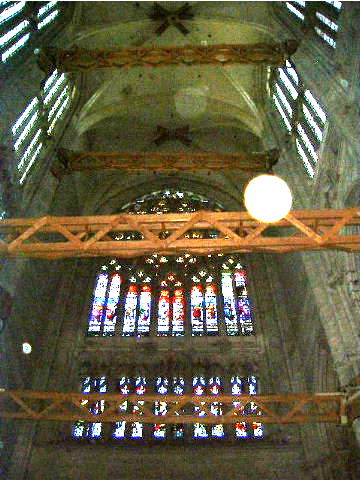
\includegraphics[totalheight=8cm]{images/beauvais_interior_supports.jpg}}
\caption{Специальные меры, предохраняющие Собор Святого Петра в Бове от разрушения}
\end{figure}
